\section{Nelder-Meadの滑降シンプレックス法}

\begin{frame}[t,fragile]{Nelder-Meadの滑降シンプレックス法}
  \begin{itemize}
    \setlength{\itemsep}{1em}
  \item 関数値のみ。導関数の情報を必要としない
  \item プログラミングが簡単
  \item 収束は遅いが、安定に極小値が求まる
  \item $N+1$個の頂点からなる$N$次元の単体(シンプレックス)を変形しながら、極小値を探す
    \begin{itemize}
    \item 2次元: 三角形
    \item 3次元: 四面体
    \end{itemize}
  \item 別名「アメーバ法」
  \end{itemize}
\end{frame}

\begin{frame}[t,fragile]{Nelder-Meadの滑降シンプレックス法}
  \begin{itemize}
    \setlength{\itemsep}{1em}
  \item $N+1$個の点$x_0,x_1,\cdots,x_N$は$f(x_0) \le f(x_1) \le \cdots \le f(x_N)$と並べられているとする
  \item 最大値を取る点$x_N$を除く$N$点の重心を$x_g$とする
  \item Nelder-Mead法では以下のステップを繰り返す
    \begin{itemize}
      \item $x_N$の$x_g$に関する対称な点と$x_N$の関数値を比較し、小さい方に移動(反射)
      \item $x_0$の関数値よりも小さくなるようであればさらに先に進む(拡大)
      \item $x_N$の関数値が$x_{N-1}$のものよりもまだ大きい場合には$x_N$を$x_g$に近づける(縮小)
      \item それでも$x_N$の関数値が小さくならない場合、$x_0$以外の点を$x_0$に一様に近づける(収縮)
    \end{itemize}
  \end{itemize}
\end{frame}

\begin{frame}[t,fragile]{Nelder-Meadの滑降シンプレックス法}
  \vspace*{-2em}
  \hspace*{1em}\resizebox{!}{1.0\textheight}{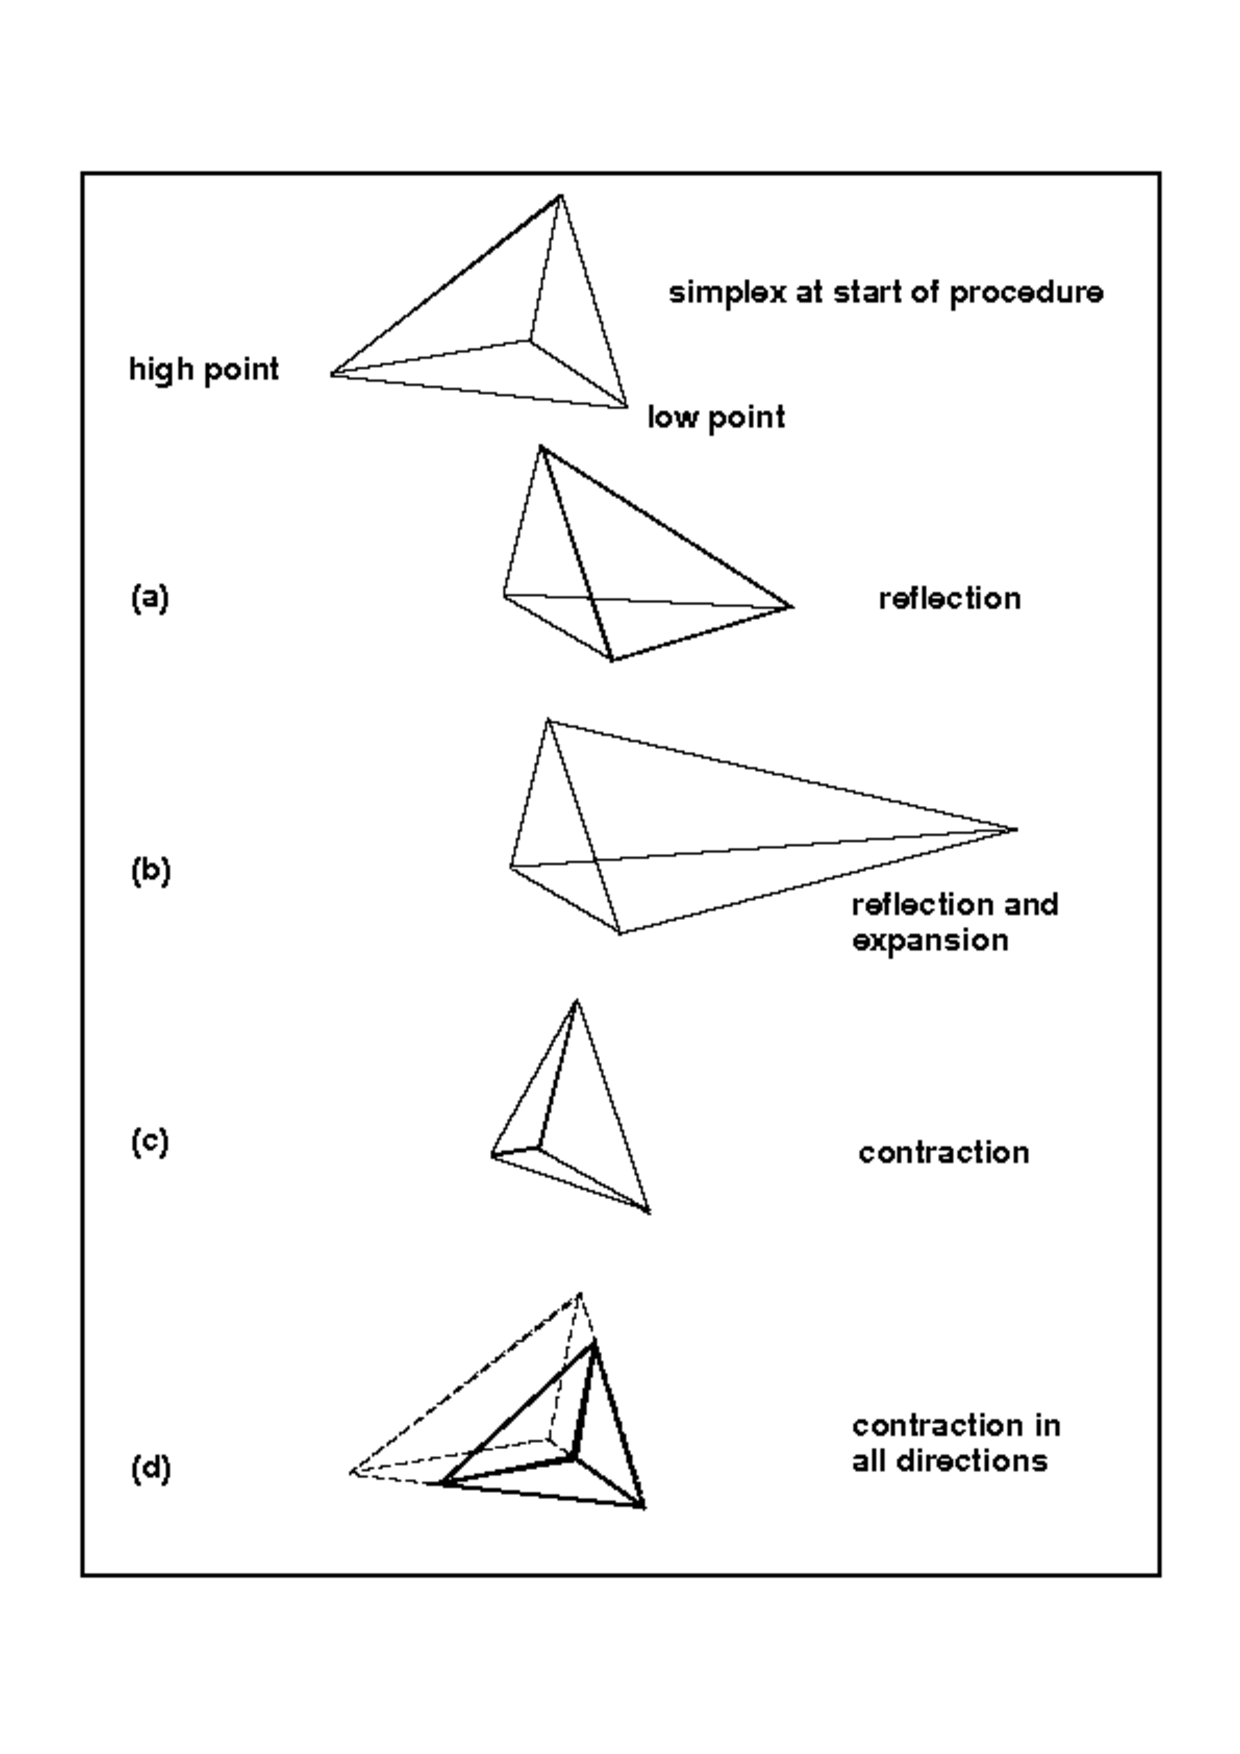
\includegraphics{image/neldermead.pdf}}

  \vspace*{-4em}
  \hspace*{16em}{\tiny\url{http://www.kniaz.net/software/RosNM.aspx}}
\end{frame}
